% -----------------
%  UNIVERSITY OF LIMERICK

% Template for Undergrad/Master/PhD Thesis
% -----------------
%Refresh the tex project by running the following commands in the terminal:
% rm *.glo *.gls *.glsdefs *.acn *.acr *.alg *.bbl *.blg *.lof *.lot *.out *.toc

% pdflatex thesis
% makeglossaries thesis or bibtex thesis 
% pdflatex thesis
% pdflatex thesis
% ------------------
% Giuseppe Torre 2020
% Department of Computer Science - University of Limerick
% Also here: https://zenodo.org/record/3908239#.XvWuo_ko_6p/ 

% Based on Harish Bhanderi's PhD/MPhil template, then Uni Cambridge http://www-h.eng.cam.ac.uk/help/tpl/textprocessing/ThesisStyle/ corrected and extended in 2007 by Jakob Suckale, then MPI-CBG PhD programme  and made available through OpenWetWare.org - the free biology wiki corrected and extended   
% ------------------


%: Style file for Latex
% Most style definitions are in the external file PhDthesisPSnPDF.
% In this template package, it can be found in ./Latex/Classes/
\documentclass[twoside,12pt, openany]{Latex/Classes/PhDthesisPSnPDF}

\usepackage{natbib}
\usepackage{url}
\usepackage{alltt} 
\usepackage{multirow}
\usepackage{color}
\usepackage{tikz}
\usetikzlibrary{positioning}
\usepackage{pgfplots}
\usepackage{tabularx}
\pgfplotsset{compat=1.18}

\usepackage[acronym]{glossaries}
\makeglossaries

%%%USE TABLE LIKE STYLING FOR GLOSSARY
% \newglossarystyle{tableacronyms}{%
%   \setglossarystyle{long}%
%   \renewenvironment{theglossary}%
%     {\begin{longtable}{@{}l p{\dimexpr\linewidth-2\tabcolsep-1em}@{}}}%
%     {\end{longtable}}%
%   % no \renewcommand{\glossentry} here
% }

%%FIXED ACRONYM HYPERLINK wasn't working (BUG) - issue - hyperlink jumped to the start of the doc
\newglossarystyle{tableacronyms}{
  \setglossarystyle{long}
  \renewenvironment{theglossary}
    {\begin{longtable}{@{}l p{\dimexpr\linewidth-2\tabcolsep-1em}@{}}}
    {\end{longtable}}
  \renewcommand*{\glossentry}[2]{%
    \glsentryitem{##1}%   
    \glstarget{##1}{\textbf{\glsentryshort{##1}}} & \glsentrylong{##1} \\%
  }%
  \renewcommand*{\glspostdescription}{}%
}

\newcommand{\urlwofont}[1]
{
\urlstyle{same}\url{#1}
}

% to display Math
\usepackage{mathtools}

% to Display C++ code
\definecolor{c++red}{rgb}{0.6,0,0} % for strings
\definecolor{c++green}{rgb}{0.25,0.5,0.35} % comments
\definecolor{c++purple}{rgb}{0.5,0,0.35} % keyword
\usepackage{listings}
\lstset{language=C++}


%% Define a new 'leo' style for the package that will use a smaller font.
\makeatletter  
\def\url@leostyle{%
  \@ifundefined{selectfont}{\def\UrlFont{\sf}}{\def\UrlFont{\small\ttfamily}}}
\makeatother
%% Now actually use the newly defined style.
\urlstyle{leo}

%: Macro file for Latex
% Macros help you summarise frequently repeated Latex commands.
% Here, they are placed in an external file /Latex/Macros/MacroFile1.tex
% An macro that you may use frequently is the figuremacro (see introduction.tex)
% \include{Latex/Macros/MacroFile1} % moved below after \begin{document}



%: ----------------------------------------------------------------------
%:                  TITLE PAGE: name, degree,..t
% ----------------------------------------------------------------------
% below is to generate the title page with crest and author name

%if output to PDF then put the following in PDF header
\ifpdf  
    \pdfinfo { /Title (Prediction of Chronic Disease Risk Using Nutrition, Lifestyle and Clinical Data from TILDA)
        /Creator (Abderahman Haouit)
        /Producer (pdfTeX)
        /Author (Abderahman Haouit - 24474983@studentmail.ul.ie)
        /CreationDate (D:20250601090000)  
        /ModDate (D:YYYYMMDDhhmm)       
        /Subject (Artificial Intelligence, Machine Learning, Predictive Modelling, Ageing, Nutrition, Frailty, TILDA, Health Informatics)
        /Keywords (Machine Learning, Artificial Intelligence, TILDA, Predictive Modelling, Frailty, Nutrition, Ageing, Longitudinal Data, Healthcare Analytics)}
    \pdfcatalog { /PageMode (/UseOutlines)
        /OpenAction (fitbh)}
\fi


\title{ Prediction of Chronic Disease Risk Using Nutrition, Lifestyle \& Clinical Data from The Irish Longitudinal Study on Ageing (TILDA)}



% ----------------------------------------------------------------------
% The section below defines www links/email for author and institutions
% They will appear on the title page of the PDF and can be clicked
\ifpdf
  \author{\href{mailto: 24474983@studentmail.ul.ie}{Abderahman Haouit}}
%  \cityofbirth{born in XYZ} % uncomment this if your university requires this
%  % If city of birth is required, also uncomment 2 sections in PhDthesisPSnPDF
%  % Just search for the "city" and you'll find them.

% here the links to the Institution you belong to
  \researchcentre{\href{https://www.ul.ie/scieng/schools-and-departments/department-computer-science-and-information-systems/research-csis}{CSIS Research Centre}}
  \faculty{\href{https://www.ul.ie/scieng/schools-and-departments/department-computer-science-and-information-systems}{Department of Computer Science and Information Systems}}
  \department{\href{https://www.ul.ie/scieng}{Faculty of Science and Engineering}}
  \university{\href{http://www.ul.ie}{University of Limerick}}

  % The crest is a graphics file of the logo of your research institution.
  % Place it in ./0_frontmatter/figures and specify the width
  \crest{
\includegraphics[scale=0.45]{logonew2020.jpg}}
  
% If you are not creating a PDF then use the following. The default is PDF.
%\else
 % \author{YourName}
%  \cityofbirth{born in XYZ}
 % \collegeordept{CollegeOrDept}
  %\university{University}
  %\crest{\includegraphics[width=4cm]{logo.png}}
%\fi

%\renewcommand{\submittedtext}{change the default text here if needed}
\degree{Artificial Intelligence (MSc) 2026}
\degreedate{}


% ----------------------------------------------------------------------
       
% turn of those nasty overfull and underfull hboxes
\hbadness=10000
\hfuzz=50pt


%: --------------------------------------------------------------
%:                  FRONT MATTER: dedications, abstract,..
% --------------------------------------------------------------

\begin{document}

\include{Latex/Macros/MacroFile1}

%\language{english}



% sets line spacing
\renewcommand\baselinestretch{1.2}
\baselineskip=18pt plus1pt


%: ----------------------- generate cover page ------------------------

\maketitle  % command to print the title page with above variables


%: ----------------------- cover page back side ------------------------
% Your research institution may require reviewer names, etc.
% This cover back side is required by Dresden Med Fac; uncomment if needed.

% \newpage


 \begin{tabbing}
1.  Supervisor: \= Dr. Alison O'Connor    \\
 \>  \= Computer Science \& Information Systems\\
 \>  \= University \emph{of} Limerick \\
 \>  \= Ireland \\
 \end{tabbing}



%: ----------------------- abstract ------------------------

% Your institution may have specific regulations if you need an abstract and where it is to be placed in the document. The default here is just after title.
%: Declaration of originality

% Thesis Abstract -----------------------------------------------------
% BMRC style

%\begin{abstractslong}    %uncommenting this line, gives a different abstract heading
\begin{abstracts}        %this creates the heading for the abstract page.

\textbf{Background:} Chronic disease and functional decline are major health challenges for older adults, yet how well self-reported health burden can predict disease onset across longitudinal waves remains underexplored.

\textbf{Methods:} A longitudinal machine learning framework was developed using five waves of TILDA data (2009--2019). Four model families, \texttt{logistic Regression}, \texttt{XGBoost}, \texttt{random Forest}, and a \texttt{multi-Layer Perceptron}, were compared across a single wave baseline and two pooled multi wave designs. Performance was assessed using \gls{CV} \gls{AUC}. The contribution of individual domain-specific predictors was evaluated using a bootstrapped add-on analysis.

\textbf{Results:} Pooled multi wave modelling improved predictive performance and stability over the single wave baseline, increasing \gls{CV} \gls{AUC} from $0.589 \pm 0.072$ to $0.718 \pm 0.006$. Reducing the feature set to the 20 most important predictors caused no measurable performance loss, while cognitive, psychosocial, nutritional, and behavioural add-on variables produced no statistically significant improvement.

\textbf{Conclusions:} Among community dwelling older adults, chronic disease risk prediction was driven primarily by accumulated self-reported and functional health measures, particularly medication use, pain, and self-rated health, rather than domain specific biomarker or lifestyle profiles. These findings suggest that publicly available survey data can support meaningful risk stratification with limited feature sets.

\textbf{Keywords:} ageing, \glsentryfull{ML}, predictive modelling, chronic disease, functional decline, health burden, \glsentryfull{TILDA}, \glsentryfull{XGB}

\end{abstracts}
%\end{abstractlongs}


% ---------------------------------------------------------------------------
% ----------------------- end of thesis sub-document ------------------------
% ---------------------------------------------------------------------------
\include{0_frontmatter/declaration}


%: ----------------------- tie in front matter ------------------------

\frontmatter

% Thesis Acknowledgements ------------------------------------------------


%\begin{acknowledgementslong} %uncommenting this line, gives a different acknowledgements heading
\begin{acknowledgements}      %this creates the heading for the acknowlegments

I would like to acknowledge my supervisor, Alison O'Connor, for her guidance, support, and for providing a well organised environment as well as the necessary resources throughout the journey of this project.

I would also like to thank the \gls{UL} Science and Engineering Research Ethics Committee for approving the ethical aspects of this research. Special thanks to the \gls{ISSDA} team for facilitating access to the \gls{TILDA} dataset, collected by Trinity College Dublin.

\end{acknowledgements}
%\end{acknowledgmentslong}

% ------------------------------------------------------------------------
\include{0_frontmatter/dedication}


%: ----------------------- contents ------------------------

\setcounter{secnumdepth}{3} % organisational level that receives a numbers
\setcounter{tocdepth}{3}    % print table of contents for level 3
\tableofcontents            % print the table of contents
% levels are: 0 - chapter, 1 - section, 2 - subsection, 3 - subsection


%: ----------------------- list of figures/tables ------------------------

\listoftables  % print list of tables
\listoffigures	% print list of figures


%: ----------------------- glossary ------------------------
% \cleardoublepage
% \renewcommand{\nomname}{List of Abbreviations}
% Tie in external source file for definitions: /0_frontmatter/glossary.tex
% Glossary entries can also be defined in the main text. See glossary.tex
% this file is called up by thesis.tex
% content in this file will be fed into the main document

% Glossary entries are defined with the command \nomenclature{1}{2}
% 1 = Entry name, e.g. abbreviation; 2 = Explanation
% You can place all explanations in this separate file or declare them in the middle of the text. Either way they will be collected in the glossary.

% required to print nomenclature name to page header
\markboth{\MakeUppercase{\nomname}}{\MakeUppercase{\nomname}}

% ----------------------- contents from here ------------------------

% --- General / Study Acronyms ---
\newacronym{TILDA}{TILDA}{The Irish Longitudinal Study on Ageing}
\newacronym{ML}{ML}{Machine Learning}
\newacronym{WHO}{WHO}{World Health Organization}
\newacronym{EU}{EU}{European Union}
\newacronym{UK}{UK}{United Kingdom}
\newacronym{HRS}{HRS}{Health and Retirement Study, (a longitudinal study of ageing in the United States)}
\newacronym{SHARE}{SHARE}{Survey of Health, Ageing and Retirement in Europe}
% --- Clinical / Ageing Measures ---
\newacronym{AUC}{AUC}{Area Under the ROC Curve}
\newacronym{BMI}{BMI}{Body Mass Index}
\newacronym{TUG}{TUG}{Timed Up and Go (mobility test)}
\newacronym{MMSE}{MMSE}{Mini-Mental State Examination}
\newacronym{CESD}{CES-D}{Center for Epidemiologic Studies Depression Scale}
\newacronym{CVD}{CVD}{Cardiovascular Disease}
\newacronym{DM}{DM}{Diabetes Mellitus}
\newacronym{HTN}{HTN}{Hypertension}
\newacronym{CHD}{CHD}{Coronary Heart Disease}
\newacronym{CKD}{CKD}{Chronic Kidney Disease}
\newacronym{MCI}{MCI}{Mild Cognitive Impairment}
\newacronym{FI}{FI}{Frailty Index}
\newacronym{PA}{PA}{Physical Activity}
\newacronym{MVPA}{MVPA}{Moderate-to-Vigorous Physical Activity}
\newacronym{VPA}{VPA}{Vigorous Physical Activity}
\newacronym{UGS}{UGS}{Usual Gait Speed}
\newacronym{MGS}{MGS}{Maximum Gait Speed}
\newacronym{HGS}{HGS}{Hand Grip Strength}
\newacronym{FOF}{FOF}{Fear of Falling}
\newacronym{IADL}{IADL}{Instrumental Activities of Daily Living}
\newacronym{BADL}{BADL}{Basic Activities of Daily Living}
\newacronym{GDS}{GDS}{Geriatric Depression Scale}
\newacronym{MOCA}{MOCA}{Montreal Cognitive Assessment}
\newacronym{MRI}{MRI}{Magnetic Resonance Imaging}
\newacronym{recall}{Recall}{Recall (true positive rate)}
\newacronym{F1}{F1}{F1-score (harmonic mean of precision and recall)}   
\newacronym{MPOD}{MPOD}{Macular pigment optical density}  
\newacronym{LDA}{LDA}{Linear Discriminant Analysis}
\newacronym{DNN}{DNN}{Deep Neural Network}
\newacronym{AI}{AI}{Artificial Intelligence}
\newacronym{MLP}{MLP}{Multilayer Perceptron}
\newacronym{SVM}{SVM}{Support Vector Machine}
% --- Statistical / ML Methods ---
\newacronym{RF}{RF}{Random Forest}
\newacronym{GBM}{GBM}{Gradient Boosting Machine}
\newacronym{CV}{CV}{Cross-Validation}
\newacronym{ROC}{ROC}{Receiver Operating Characteristic}
\newacronym{HR}{HR}{Hazard Ratio}
\newacronym{OR}{OR}{Odds Ratio}
\newacronym{CI}{CI}{Confidence Interval}
\newacronym{RMSE}{RMSE}{Root Mean Squared Error}
\newacronym{PRAUC}{PR-AUC}{Precision-Recall Area Under the Curve}
\newacronym{AUROC}{AUROC}{Area Under the Receiver Operating Characteristic Curve}
\newacronym{SHAP}{SHAP}{Shapley Additive Explanations}
\newacronym{PCA}{PCA}{Principal Component Analysis} 
% \begin{multicols}{2} % \begin{multicols}{#columns}[header text][space]
% \begin{footnotesize} % scriptsize(7) < footnotesize(8) < small (9) < normal (10)
% \setlength{\nomlabelwidth}{2.5cm}

% \printnomenclature[1.5cm] % [] = distance between entry and description
% \label{nom} % target name for links to glossary
% \end{footnotesize}
% \end{multicols}
\printglossary[type=\acronymtype, title=List of Abbreviations, style=tableacronyms]
\addcontentsline{toc}{chapter}{List of Abbreviations}

%: --------------------------------------------------------------
%:                  MAIN DOCUMENT SECTION
% --------------------------------------------------------------

% the main text starts here with the introduction, 1st chapter,...
\mainmatter

% \renewcommand{\chaptername}{} % uncomment to print only "1" not "Chapter 1"


%: ----------------------- subdocuments ------------------------

% Parts of the thesis are included below. Rename the files as required.
% But take care that the paths match. You can also change the order of appearance by moving the include commands.

% this file is called up by thesis.tex
% content in this file will be fed into the main document

%: ----------------------- introduction file header -----------------------
\chapter{Introduction}

% the code below specifies where the figures are stored
\ifpdf
    \graphicspath{{1_introduction/figures/PNG/}{1_introduction/figures/PDF/}{1_introduction/figures/}}
\else
    \graphicspath{{1_introduction/figures/EPS/}{1_introduction/figures/}}
\fi

% ----------------------------------------------------------------------
%: ----------------------- introduction content ----------------------- 
% ----------------------------------------------------------------------
\section{Background and Context}
Chronic conditions—including cardiovascular disease, diabetes, and frailty—are leading contributors to morbidity and mortality in ageing populations~\cite{bencivengaAtrialFibrillationElderly2020, bardonPredictorsIncidentMalnutrition2020}. These conditions are associated with declines in functional capacity (e.g., gait speed, grip strength~\cite{davisComparisonGaitSpeed2021}), increased healthcare utilisation~\cite{mooreCountingTimeLived2017}, and reduced quality of life~\cite{huangSexDifferencesAssociations2020}.  

Traditional risk prediction models rely primarily on clinical biomarkers such as blood pressure and lipid profiles. Evidence suggests that multidimensional predictors, including nutrition~\cite{murphyPlasmaLuteinZeaxanthin2023}, physical activity~\cite{lairdPhysicalActivityDose2023}, mental health~\cite{mcdowellAssociationsPhysicalActivity2018}, and social determinants~\cite{mccrorySocialDisadvantageSocial2016}, improve predictive performance.

The Irish Longitudinal Study on Ageing (\gls{TILDA}) provides a nationally representative dataset of adults aged 50+ in Ireland with repeated measures across multiple domains. The Harmonized \gls{TILDA} dataset aligns variables with the RAND Health and Retirement Study (\gls{HRS}) framework for cross-country comparability, while the raw waves contain additional study-specific variables. The IDS dataset supplements coverage for participants with disabilities.  

These data motivate the development of integrated models combining traditional (e.g., blood pressure, cholesterol, diabetes diagnosis) and non-traditional (e.g., nutrition biomarkers, physical activity, mental health, social determinants) risk factors. This thesis focuses on the non-traditional predictors to quantify their added predictive value.

% ----------------------------------------------------------------------
% Research Problem
\section{Research Problem and Motivation}
Existing \gls{ML} approaches for chronic disease prediction in older adults face several challenges:

\subsection{Limited Integration of Multidimensional Data}
Most models prioritise clinical variables but neglect modifiable lifestyle and nutrition factors~\cite{murphyPlasmaLuteinZeaxanthin2023, lairdPhysicalActivityDepression2023}.

\subsection{Underuse of Longitudinal Dynamics}
Few studies exploit repeated measures to capture trajectories of risk, such as frailty progression~\cite{moguilnerImportanceAgePrediction2021}.

\subsection{Lack of Explainability}
Many \gls{ML} models are not interpretable, limiting clinical utility~\cite{donoghueUsingConditionalInference2023}.

Addressing these gaps requires methods that integrate multidomain predictors, account for longitudinal dynamics, and balance predictive accuracy with interpretability.

% ----------------------------------------------------------------------
% Research Aims
\section{Research Aims and Objectives}
This thesis develops and validates \gls{ML} models that integrate nutrition, lifestyle, and mental health features with clinical data to improve prediction of chronic disease and ageing-related outcomes.

\begin{itemize}
  \item Conduct a literature review on \gls{ML} for chronic disease prediction in ageing populations, emphasising gaps in lifestyle and nutrition integration.
  \item Preprocess and harmonise \gls{TILDA} waves 1--5 and engineer multidomain features (nutrition, activity, mobility, mental health, clinical indicators).
  \item Develop and compare baseline statistical models (logistic regression) with advanced \gls{ML} methods (\gls{RF}, \gls{GBM}).
  \item Evaluate models using discrimination (\gls{AUC}), calibration, and error metrics (accuracy, precision, recall, F1-score); perform ablation analyses to quantify added value of lifestyle and nutrition.
  \item Identify actionable predictors (e.g., vitamin D status, gait speed reserve) and highlight modifiable risk factors for intervention.
  \item Document ethical, governance, and reproducibility practices for handling longitudinal pseudonymised health data.
\end{itemize}

% ----------------------------------------------------------------------
% Methodology Overview (concise, non-repetitive)
\section{Methodology Overview}
This section summarises the workflow; detailed methods are presented in Chapter 3.  

Data are derived from both raw \gls{TILDA} waves 1--5 and the Harmonized \gls{TILDA} dataset, aligned to the \gls{HRS} framework. IDS data complements coverage for participants with disabilities.  

Missing data are addressed with complete-case analysis and multiple imputation. Derived features capture multidimensional predictors:
\begin{itemize}
    \item Frailty indices (e.g., Fried’s phenotype, \gls{FI})
    \item Mobility measures (e.g., \gls{TUG}, gait speed, grip strength)
    \item Mental health scales (e.g., \gls{CESD}, \gls{GDS})
    \item Nutrition scores (e.g., dietary diversity indices, micronutrient biomarkers)
\end{itemize}

Baseline (logistic regression) and advanced \gls{ML} models (\gls{RF}, \gls{GBM}) are tuned via cross-validation. Performance is evaluated using discrimination (\gls{AUC}), calibration (plots, Brier score), and error metrics. Explainability is assessed with feature importance and \gls{SHAP} values.

% ----------------------------------------------------------------------
% Contributions
\section{Contributions of the Research}
\begin{itemize}
  \item \textbf{Empirical:} Quantifies the predictive value of nutrition and lifestyle features beyond clinical baselines.
  \item \textbf{Methodological:} Provides a reproducible pipeline for harmonising longitudinal \gls{TILDA} data and integrating multidomain features into \gls{ML} models.
  \item \textbf{Clinical:} Highlights modifiable predictors for targeted interventions and policy to promote healthy ageing.
\end{itemize}

% ----------------------------------------------------------------------
% Thesis Outline
\section{Thesis Outline}
\begin{itemize}
    \item \emph{Chapter Two:} Literature review on \gls{ML} prediction of chronic disease in ageing populations.
    \item \emph{Chapter Three:} \gls{TILDA} study design, data preprocessing, harmonisation, and feature engineering.
    \item \emph{Chapter Four:} Modelling framework, including baseline and advanced \gls{ML}, hyperparameter tuning, validation, and evaluation metrics.
    \item \emph{Chapter Five:} Results, model comparison, feature importance, and ablation analyses.
    \item \emph{Chapter Six:} Discussion of implications, limitations, ethical considerations, and future work.
\end{itemize}

\vspace{5 mm}

A series of documents have been included in the Appendix section of this dissertation. These are:

\begin{itemize}
\item \emph{Appendix A}: Variable codebook and wave harmonisation notes (including anonymisation actions, top-coding, and grouping rules relevant to the features used).
\item \emph{Appendix B}: Ethics.
\item \emph{Appendix C}: Modelling details, additional tables/figures, and reproducibility checklist (overview of data processing scripts).
\end{itemize} 

\vspace{5 mm}

A digital archive is attached to this dissertation containing:(Access request required)

\begin{itemize}
\item \emph{folder 1}: Preprocessing and feature-engineering scripts (documentation only; no raw \gls{TILDA} data).
\item \emph{folder 2}: Model training/evaluation code and configuration files to reproduce reported results.
\end{itemize}	
% this file is called up by thesis.tex
% content in this file will be fed into the main document

%: ----------------------- name of chapter  -------------------------

\chapter{Literature Review} % top level followed by section, subsection

%: ----------------------- paths to graphics ------------------------

% change according to folder and file names
\ifpdf
    \graphicspath{{2_chapter2/figures/PNG/}{2_chapter2/figures/PDF/}{2_chapter2/figures/}}
\else
    \graphicspath{{2_chapter2/figures/EPS/}{2_chapter2/figures/}}
\fi

%: ----------------------- contents from here ------------------------

\section{Introduction} 
\begin{itemize}
    \item Purpose of this chapter
    \item Brief overview on TILDA as a unique dataset (rich, longitudinal, multi-domai...)
    \item Scope: frailty, mental health, chronic disease, multimorbidity, nutrition, and ML models
\end{itemize}

\section{Chronic Disease and Ageing}
\begin{itemize}
    \item The burden of chronic conditions in older adults
    \item Healthy ageing framework \gls{WHO}
    \item Importance of multimorbidity, frailty, mental health
\end{itemize}

\subsection{Frailty and Physical Function}
\begin{itemize}
    \item Gait speed, grip strength, functional mobility decline 
    \item Predictors of frailty transitions (\cite{mccarthyAssociationMetabolicSyndrome2023}, \cite{huangAgeModifyAssociations2019}, \cite{oconnellOrthostaticHypotensionOrthostatic2015})
\end{itemize}

\subsection{Mental Health in Older Adults}
\begin{itemize}
    \item Depression, anxiety, loneliness, social connectedness (\cite{santiniProtectivePropertiesActBelongCommit2017}, \cite{Symposia2011}, \cite{briggsWishLaterLife2021})
    \item Links between physical activity and depression (\cite{mcdowellAssociationsPhysicalActivity2018}, \cite{lairdPhysicalActivityDose2023}, \cite{lairdPhysicalActivityDepression2023})
\end{itemize}

\subsection{Nutrition and Biological Ageing}
\begin{itemize}
    \item Vitamin D, lutein, zeaxanthin, \gls{MPOD} (\cite{murphyPlasmaLuteinZeaxanthin2023}, \cite{mccarthyAssociationVitaminDeficiency2022}, lairdVitaminDeficiencyIreland2020, feeneyLowMacularPigment2013)
    \item Malnutrition and its predictors (\cite{bardonPredictorsIncidentMalnutrition2020})
    \item Biological vs chronological ageing (\cite{mccarthyMetabolicSyndromeAccelerates2023}, \cite{aziziEvidenceAssociationAllostatic2024})
\end{itemize}

\section{Machine Learning in Ageing and Chronic Disease}
\begin{itemize}
    \item Overview: Why ML is valuable in ageing research \cite{zhangMachineLearningModels2025}
    \item Transition from regression-based models → ensemble ML → deep learning(cite a example here)
\end{itemize}

\subsection{Feature Sets in ML Studies}
\begin{itemize}
    \item Clinical, sociodemographic, lifestyle, cognition, psychosocial
    \item Over-reliance on physical health predictors vs underuse of nutrition/social variables
\end{itemize}

\subsection{ML Models Used}
\begin{itemize}
    \item Logistic regression, Markov models, \gls{LDA} (traditional)
    \item Ensembles \gls{RF}, \gls{GBM}, \gls{DNN} – e.g., (\cite{xuTailoredMachineLearning2023}) diabetes prediction
    \item Unsupervised clustering for dementia (\cite{bayeneleonoreUnsupervisedMachineLearning2018})
    \item Brain age prediction models (\cite{boyleBrainpredictedAgeDifference2021}, \cite{a.shirsathSlowerSpeedBlood2024})
\end{itemize}

\subsection{Performance and Validation}
\begin{itemize}
    \item \gls{AUC}, R² ranges across tasks (diabetes, gait speed, mortality, depression)
    \item Limitations: internal validation only, cross-sectional data, no generalisation
\end{itemize}

\subsection{Explainability in ML for Ageing}
\begin{itemize}
    \item \gls{SHAP}, TreeExplainer examples (\cite{xuTailoredMachineLearning2023}, \cite{davisLinearRegressionbasedMachine2021}, \cite{davisComparisonGaitSpeed2021})
    \item Challenges of black-box models in clinical practice
\end{itemize}

\section{Gaps in the Literature}
\begin{itemize}
    \item Limited population diversity (mostly Irish, 50+)
    \item Over-reliance on physical predictors; neglect of nutrition, social, religious/spiritual, environmental variables
    \item Dominance of regression models; limited advanced ML such as neural networks, transformers
    \item Validation gaps – very few external validations, especially for ensemble and brain-age models
    \item Underexplored outcomes: pain, sleep, QoL
    \item Cross-sectional bias; weak time-series modelling
    \item Poor transparency on missing data handling
    \item Limited integration of nutrition biomarkers
    \item Lack of biological age prediction vs chronological
    \item Interpretability challenges in ML
\end{itemize}

\section{Chapter Summary}
\begin{itemize}
    \item I need to recap the main findings from LR systematic mapping excel file
    \item Identify your contribution niche:
    \begin{itemize}
        \item integrating nutrition + lifestyle + clinical predictors
        \item ML + explainability
        \item time-based prediction (longitudinal TILDA data)
    \end{itemize}
    \item Lead into Methodology (Chapter 3)
\end{itemize}



% ---------------------------------------------------------------------------
%: ----------------------- end of thesis sub-document ------------------------
% ---------------------------------------------------------------------------


% this file is called up by thesis.tex
% content in this file will be fed into the main document

\chapter{Technical Approach} \label{ch:chapter3} % top level followed by section, subsection

\ifpdf
    \graphicspath{{3_chapter3/figures/PNG/}{3_chapter3/figures/PDF/}{3_chapter3/figures/}}
\else
    \graphicspath{{3_chapter3/figures/EPS/}{3_chapter3/figures/}}
\fi

% ----------------------- contents from here ------------------------
\section{Study Design}

\gls{TILDA} provides longitudinal data across five waves for community dwelling adults in Ireland. This thesis uses data from five core \gls{TILDA} waves (Waves 1--5). For contextual comparison and benchmarking against international cohorts (see Chapter~\ref{ch:chapter1}) however, it is important to note this is an external resource and not the output of the thesis's primary preprocessing pipeline. The primary analytical work focuses on the full five wave \gls{TILDA} dataset.

\section{Cohort Definition}

All participants who provided data in at least one \gls{TILDA} wave were considered eligible. To maximise the available sample for machine learning, no exclusions were applied on the basis of age, medical conditions, mobility, cognitive status, or health centre attendance.

Participants were removed only when, after the combined manual filtering and automated preprocessing pipeline, they had no remaining usable variables. Filtering therefore occurred primarily at the \emph{variable level}, with features removed for extreme missingness, lack of variation, or non informative structure (see Chapter~\ref{ch:chapter4}). This approach preserves the largest possible sample while ensuring all retained inputs are analytically meaningful.

\subsection{Cohort inclusion criteria}
\begin{itemize}
    \item \textbf{Participant inclusion:} All respondents who contributed data in at least one wave were included in the initial sample.
    \item \textbf{Usable data requirement:} Participants were excluded only when, after manual filtering and preprocessing, no usable variables remained.
    \item \textbf{Longitudinal retention:} Individuals were retained regardless of how many waves they contributed to, enabling initial maximum dataset utilisation.
    \item \textbf{No clinical exclusions:} No participant was removed due to medical diagnoses, cognitive scores, functional limitations, or non attendance at the health centre assessment.
\end{itemize}
This approach prioritises data integrity and sample size for machine learning applications rather than clinical eligibility criteria common in classical epidemiological analyses.

\section{Data Collection}

Data used in this thesis were collected across five waves:
\begin{itemize}
    \item \textbf{Wave 1:} 2009--2011
    \item \textbf{Wave 2:} 2012--2013
    \item \textbf{Wave 3:} 2014--2015
    \item \textbf{Wave 4:} 2016--2018
    \item \textbf{Wave 5:} 2018--2020
\end{itemize}

All \gls{TILDA} data were pseudonymised prior to release. Each participant received a unique identifier (`id') along with household and cluster identifiers (`household', `cluster') to permit longitudinal linkage while preserving anonymity. Each wave included three primary components:
\begin{enumerate}
    \item \textbf{\gls{CAPI}:} Home based, computer assisted personal interviews covering health, socio demographics, and family.
    \item \textbf{\gls{SCQ}:} Paper based self completion questionnaires capturing sensitive information on mental health, lifestyle, and wellbeing.
    \item \textbf{Health Assessment:} Clinical and biomarker measurements conducted in dedicated centers or at home (Wave 1 and Wave 3).
\end{enumerate}

\subsection{Data Overview}
Before processing, raw \gls{TILDA} datasets were manually inspected, and clearly non informative variables (e.g., administrative identifiers, constant columns, high missingness) were removed. Table~\ref{tab:raw_dataset_shape} shows the raw dimensions of each dataset.

\begin{table}[htbp]
\centering
\caption{Dimensions of Raw \gls{TILDA} and Harmonised Datasets (Pre Filtering)}
\label{tab:raw_dataset_shape}
\begin{tabular}{|c|c|c|}
\hline
\textbf{Dataset} & \textbf{Participants (N)} & \textbf{Raw Variables (N)} \\
\hline
Wave 1 & 8501 & 1619 \\
Wave 2 & 7206 & 724 \\
Wave 3 & 6397 & 1029 \\
Wave 4 & 5713 & 990 \\
Wave 5 & 4978 & 983 \\
Harmonised \gls{RAND} & 8501 & 572 \\
\hline
\end{tabular}
\end{table}

\subsection{Variable filtering criteria}
Manual filtering used rules-of-thumb prior to automated cleaning:
\begin{itemize}
    \item \textbf{Missingness:} Drop variables with $>80\%$ missing values.
    \item \textbf{Unique values:} Drop variables with a single value, flag small cardinality variables (2--10 unique values) for retention.
    \item \textbf{Dominant category:} Flag variables with extremely frequent categories (e.g., $>90\%$) for review.
    \item \textbf{Identifiers / administrative fields:} Obvious IDs, version tags, and sampling weights were identified using the \gls{PMF} metadata. Variable names and descriptions were exported from each wave's \gls{PMF} file into CSV files (code provided in Appendix~\ref{app:pmf_code} ) to systematically document and review features prior to filtering. This ensured analytic relevance and traceability.
\end{itemize}

These manual checks produced a reduced variable set, subsequently processed using the automated six scenario cleaning engine (Chapter~\ref{ch:chapter4}).

\subsection{Variable filtering flowchart}
Figure~\ref{fig:variable_filter_criteria} shows the stepwise variable filtering process. This flowchart guided the removal or flagging of variables based on missingness, low variation, dominant categories, or irrelevance. Dimensionality reduction improved interpretability while preserving longitudinal structure for feature engineering and machine learning.

\begin{figure}[htbp]
\centering

\includegraphics[height=1.25\textwidth]{variable_filter_criteria.png}
\caption{Flowchart of the manual variable filtering criteria. Placeholder counts indicate remaining variables per dataset after each step.}
\label{fig:variable_filter_criteria}
\end{figure}

\section{Thematic Grouping}

After manual filtering, retained variables were organised into six thematic domains aligned with ageing literature and study objectives. The grouping process followed the standard \gls{PMF} naming conventions (Table~\ref{tab:pmf_prefixes}). Specifically, each variable's prefix indicated its data source or domain, which allowed us to systematically assign variables to one of six thematic domains. This ensured that features included in each domain were conceptually coherent and analytically meaningful. 

\subsection{Derived variable prefixes}

To systematically process \gls{TILDA} variables, each variable was assigned a prefix indicating its data source or research domain. Variables collected through the home based \gls{CAPI} follow a two letter module code plus three digit question code format (e.g., \texttt{ph121}). For questions with multiple responses or loops across participants or objects, an underscore and number indicates the specific response or loop iteration (e.g., \texttt{ph201\_05}).

Variables from the self completion questionnaire (\gls{SCQ}) are prefixed with `\gls{SCQ}'. Derived variables, constructed from either \gls{CAPI} or \gls{SCQ} data, use an uppercase code corresponding to the research area (Table~\ref{tab:pmf_prefixes}). These prefixes provide a consistent framework for categorising variables and underpin the subsequent assignment of features into thematic domains for downstream analysis.

\begin{table}[htbp]
\centering
\caption{PMF Derived Variable Prefixes and Research Areas (\cite{tilda2023pmf})}
\label{tab:pmf_prefixes}
\begin{tabular}{|l|l|}
\hline
\textbf{Variable Prefix} & \textbf{Research Area} \\
\hline
ADL & Activities of daily living \\
BEH & Health behaviours \\
BLOODS & Blood sample results \\
BP & Blood pressure \\
COG & Cognitive scales and questions \\
CRT & Choice reaction time \\
DIS & Disability, functional impairment, helpers \\
FR & Frailty, gait, exercise, falls \\
G2G & Gateway to Global Aging Data \\
GRIP & Grip strength \\
IADL & Instrumental activities of daily living \\
INC & Income variables \\
MD & Medication data \\
MH & Mental health scales and questions \\
SCR & Screening tests \\
SES & Socio-economic class variables \\
SOC & Social support and relationships \\
\hline
\end{tabular}
\end{table}

\subsection{Feature groups}

Using the \gls{PMF} prefixes as a guide, variables were systematically mapped to six thematic groups (Table~\ref{tab:feature_groups}). Each thematic group captures a conceptually coherent domain, reflecting physical, cognitive, social, and behavioural aspects of ageing. This categorisation served two key purposes in the thesis: 

1. It structured the data for the automated six scenario cleaning engine (Chapter~\ref{ch:chapter4}), ensuring consistent application of filtering rules and facilitating reproducible preprocessing.

2. It aligned feature selection with the analytic focus of the thesis, enabling machine learning models to leverage variables that are both conceptually meaningful and longitudinally robust across multiple waves.

The six thematic groups integrate information from \gls{CAPI}, \gls{SCQ}, and derived variables, covering socio demographic context, physical health, functional status, lifestyle behaviours, nutrition/metabolic biomarkers, and psychological/cognitive measures. This structured grouping enhances interpretability, ensures comprehensive domain coverage, and provides a foundation for downstream predictive modelling and risk assessment.

\begin{table}[htbp]
\centering
\caption{Thematic grouping of longitudinal features}
\label{tab:feature_groups}
\begin{tabular}{|c|p{4cm}|p{5cm}|p{5cm}|}
\hline
\textbf{ID} & \textbf{Thematic Group} & \textbf{Description} & \textbf{Representative Variables} \\
\hline
1 & Socio Demographic \& Context & Baseline stratification factors & Age, Gender, Education, \gls{INC}, Marital Status, \gls{SOC} \\
2 & Physical Health \& Clinical Baseline & Self reported and clinical indicators & Self Rated Health \gls{SCR}, \gls{BMI}, \gls{BP}, Comorbidity Count \gls{MD} \\
3 & Functional Status \& \gls{FR} & Measures of mobility and physical decline & \gls{FR} Index \gls{FR}, \gls{UGS}, Falls History \textit{SCQFalls}, \gls{IADL} \gls{DIS} \\
4 & Lifestyle \& Behavioural & Modifiable health related behaviours & Smoking, Alcohol Intake \textit{SCQAlco}, \gls{PA} \gls{IPAQ} \\
5 & Nutrition \& Metabolic Biomarkers & Objective nutritional and metabolic markers & Plasma Carotenoids, Lutein, Zeaxanthin, Vitamin D/B12, Cholesterol \\
6 & Psychological \& Cognitive & Mental health and cognitive performance & \gls{CESD}, Loneliness \textit{MHucla}, \gls{COG}, \gls{CRT} \\
\hline
\end{tabular}
\end{table}			
% this file is called up by thesis.tex
% content in this file will be fed into the main document

\chapter{Implementation Details} \label{chap:Implementation Details} % top level followed by section, subsection


% ----------------------- paths to graphics ------------------------

% change according to folder and file names
\ifpdf
    \graphicspath{{4_chapter4/figures/PNG/}{4_chapter4/figures/PDF/}{4_chapter4/figures/}}
\else
    \graphicspath{{4_chapter4/figures/EPS/}{4_chapter4/figures/}}
\fi


% ----------------------- contents from here ------------------------

\section{Data Preprocessing}

The primary aim of preprocessing was to convert all features, regardless of their original datatype (numeric, categorical, text based, or mixed formats), into a standardised numerical representation suitable for machine learning. All non response and sentinel values were consistently mapped to $\texttt{-1.0}$, and all valid values were converted to $\texttt{float64}$. This ensured compatibility across the five \gls{TILDA} waves and enabled uniform downstream feature engineering and modelling.
\subsection{Data Overview}
% explain this is what we have after teh mnual cleaing described in chapter 3 we used this to visuaise in depth etc etc and tehne went on to clean...
\begin{table}[htbp]
\centering
\caption{Dimensions (Rows and Features) of Raw and Harmonised Datasets}
\label{tab:dataset_shape}
\begin{tabular}{|c|c|c|}
\hline
\textbf{Dataset} & \textbf{Row (participants)} & \textbf{Column (variables)} \\
\hline
Wave 1 & 8501 & 809 \\
Wave 2 & 7206 & 482 \\
Wave 3 & 6397 & 639 \\
Wave 4 & 5713 & 592 \\
Wave 5 & 4978 & 577 \\
Harmonised & 8501 & 453 \\
\hline
\end{tabular}
\end{table}

\subsection{Cleaning Engine}

The preprocessing strategy was built around a systematic classification of raw variable types. An exploratory audit across the five waves revealed nine distinct data scenarios (summarised in Appendix~\ref{tab:cleaning_scenario_tables}), ranging from simple numeric fields to complex multi-class string hybrids. The challenge was not merely to clean variables, but to construct a reproducible pipeline that produced \emph{numerical homogeneity} across all waves.

To accomplish this, the nine scenarios were organised into a \emph{Six-Step Cleaning Engine}. The steps reflect a principle of cumulative simplification: resolving simple and unambiguous cases first increases the proportion of clean numerical variables before addressing more complex structures.

\begin{itemize}
    \item \textbf{Steps 1–2: Missingness and sentinel standardisation.} These steps ensured consistent encoding of \texttt{-1.0} across all waves.
    \item \textbf{Step 3: Numeric recovery.} Units, symbols, and censored numeric strings (e.g., ``50+'') were stripped and converted.
    \item \textbf{Steps 4–6: Categorical complexity.} Ordinal, binary, and multi-class textual variables were processed in order of transformation confidence, with Step 6 applying the most general parsing rules.
\end{itemize}

This structured sequence ensured that each wave passed through the same deterministic cleaning logic. Figure~\ref{fig:cleaning_flow} shows the flow of the pipeline.

% --- FIGURE ---
\begin{figure}[htbp]
\centering
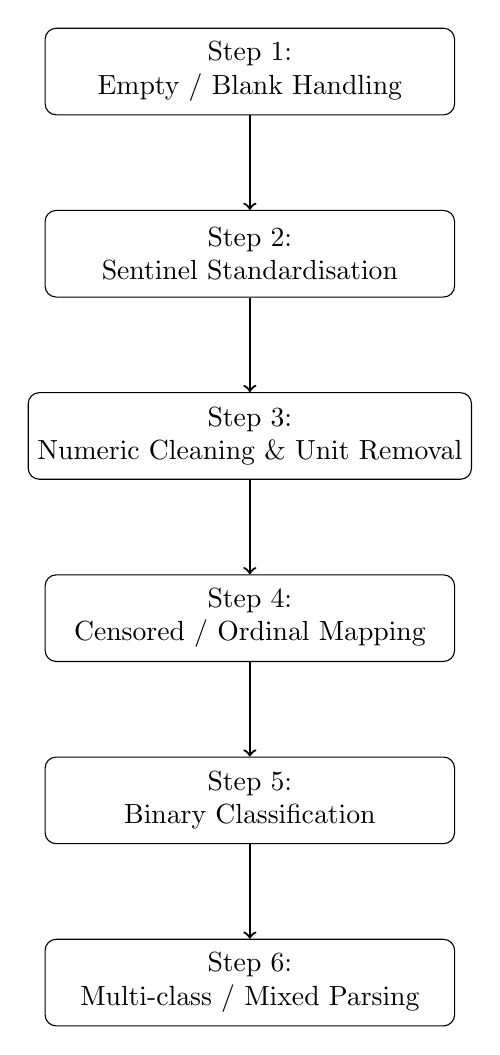
\begin{tikzpicture}[
    node distance=12mm,
    every node/.style={rectangle, rounded corners, draw=black, align=center, minimum width=5.2cm, minimum height=1.1cm}
]

\node (step1) {Step 1:\\Empty / Blank Handling};
\node (step2) [below=of step1] {Step 2:\\Sentinel Standardisation};
\node (step3) [below=of step2] {Step 3:\\Numeric Cleaning \& Unit Removal};
\node (step4) [below=of step3] {Step 4:\\Censored / Ordinal Mapping};
\node (step5) [below=of step4] {Step 5:\\Binary Classification};
\node (step6) [below=of step5] {Step 6:\\Multi-class / Mixed Parsing};

\draw[->, thick] (step1) -- (step2);
\draw[->, thick] (step2) -- (step3);
\draw[->, thick] (step3) -- (step4);
\draw[->, thick] (step4) -- (step5);
\draw[->, thick] (step5) -- (step6);

\end{tikzpicture}
\caption{Flowchart of the Six-Step Cleaning Pipeline applied to all \gls{TILDA} waves. See count tables in Appendix~\ref{tab:cleaning_scenario_tables} for detailed scenario progression at each step.}
\label{fig:cleaning_flow}
\end{figure}

\begin{enumerate}
    \item \textbf{Empty / Blank Values:} Converts all \texttt{NaN}, empty strings, and whitespace to \texttt{-1.0}.
    \item \textbf{Sentinel Values:} Standardises wave specific non-response codes (e.g., $-98, -99$) to \texttt{-1.0}.
    \item \textbf{Numeric Transformation:} Removes non-numeric characters and converts censored or annotated values to numerical equivalents.
    \item \textbf{Censored Categorical:} Applies known ordinal transformations (e.g., health scales, Likert ranges).
    \item \textbf{Binary Categorical:} Automatically maps two level variables (e.g., Yes/No, Male/Female) to \texttt{0.0/1.0}.
    \item \textbf{Multi-Class / Mixed:} Applies text parsing, numerical extraction, and rule based mappings to remaining multi-class variables.
\end{enumerate}

\section{Data Integration and Longitudinal Alignment}

Following cleaning, features were aligned across waves based on:

\section{Summary}

This chapter detailed the preprocessing pipeline applied to the five \gls{TILDA} waves. The approach centred on a reproducible Six-Step Cleaning Engine, combined with systematic wave-to-wave standardisation and thematic feature organisation. These steps produced a structured dataset suitable for longitudinal analysis and machine learning modelling. No cross-cohort harmonisation was performed; any references to a “Harmonised” dataset refer solely to the external RAND Harmonised TILDA.





% ---------------------------------------------------------------------------
% ----------------------- end of thesis sub-document ------------------------
% ---------------------------------------------------------------------------
%: ---------------------------------------------------------------------------
%: CHAPTER 5: EMPIRICAL EVALUATION
%: ---------------------------------------------------------------------------
\chapter{Empirical Evaluation}\label{ch:chapter5}

\section{Modeling and Evaluation Framework}
This section specifies how models were constructed and evaluated in this chapter, including the final analysis samples, outcome definitions, modelling designs, and evaluation procedures, building on the data preparation described in Chapters~\ref{ch:chapter3} and~\ref{ch:chapter4}.

For all incident prediction, the outcome is defined per task and transition (see Section~5.1.1). Individuals with the target condition present at the start of a transition were excluded so that only at-risk observations contributed to model training and evaluation. This rule was applied consistently across all designs and for both Track A (composite outcome) and Track B (disease-specific outcomes).

Final analysis samples differed by design due to data structure. The baseline design (D1) uses a single transition (Wave 1$\rightarrow$Wave 5). The pooled multi-wave designs (D2 and D3) aggregate all eligible consecutive transitions (e.g., W1$\rightarrow$W2, W2$\rightarrow$W3, W3$\rightarrow$W4, W4$\rightarrow$W5), allowing participants to contribute multiple at-risk observations. Sample sizes and incident rates are summarised in Table~5.1.

\begin{table}[ht]
\centering
\caption{Analysis samples by modelling design}\label{tab:analysis_samples}
\resizebox{\textwidth}{!}{
\begin{tabular}{|l|c|c|c|}
\hline
\textbf{Design} & \textbf{Observations (n)} & \textbf{Incident cases (n)} & \textbf{Incidence rate (\%)} \\ \hline
D1: Baseline (W1$\rightarrow$W5) & 916 & 248 & 27.07 \\ \hline
D2: Multi-wave pooled & 14{,}296 & 3{,}212 & 22.5 \\ \hline
D3: Top-20 (pooled) & 14{,}296 & 3{,}212 & 22.5 \\ \hline
\end{tabular}
}
\end{table}

\subsection{Outcome Definitions (Track A and Track B)}
Two complementary prediction tasks were defined.

\begin{enumerate}
	\item \textbf{Track A:} Focused on incident chronic disease as a composite binary outcome. This was operationalised using a harmonised indicator (ICD10\_ANY), defined as the first occurrence of any chronic disease recorded across follow-up waves. Individuals were labelled as 1 if an incident diagnosis occurred and 0 if they remained disease-free throughout the observation period. 
	\item \textbf{Track B:} Focused on disease-specific prediction tasks. Separate models were developed for individual conditions, including circulatory disease (ICD10\_09), diabetes (ph726\_01), and related outcomes. For each task, the outcome was defined as the first recorded diagnosis of the specific condition, with participants excluded if the condition was present at the baseline of the corresponding transition.
\end{enumerate}	

All outcome variables were harmonised across waves to ensure consistency. Incident status was defined strictly based on the absence of the condition at baseline and its occurrence at follow-up, ensuring temporal validity of the prediction task. % placeholer:add a mention for the variables mentioned in thesis we need to add them to appendix showing the feature, label and encoded values for the outcome definitions. This will be important for reproducibility and transparency, especially for Track B where multiple disease-specific outcomes are modelled.

% Placeholder: Table of outcome definitions and coding rules for all modeled conditions.

\subsection{Modelling Designs} % why didnt we mention ph003 etc it played a roll in the clasisfiairton of who is freee of disease at baseline and who is not. We can add a table in the appendix showing the variables used to define the outcome and the coding rules for each condition. especially for d2 and d3used ph003 consitley d1 didnt important to shoscase is the use of the variable for defining the outcome and the at-risk population.
Three primary modelling designs were implemented to address distinct analytical objectives:

\begin{itemize}
	\item \textbf{D1 (Baseline):} Models trained on a single transition from Wave 1 (baseline) to Wave 5 (follow-up), using only participants free of the outcome at baseline.
	\item \textbf{D2 (Multi-wave pooled):} Models trained on pooled consecutive transitions (e.g., W1$\rightarrow$W2, W2$\rightarrow$W3, etc.), allowing participants to contribute multiple transitions if they remained at risk. This design leverages longitudinal structure to increase sample size and capture temporal dynamics.
	\item \textbf{D3 (Top-20 features):} A reduced version of D2 but restricted to the 20 most informative predictors identified using XGBoost gain importance, enabling evaluation of model simplicity and feature efficiency. 
\end{itemize}

Track B (disease-specific) models followed the D2 or D3 design, with XGBoost as the primary model family due to its superior performance and flexibility in handling class imbalance and feature interactions.

Each design was chosen to address specific research questions: D1 for baseline prediction, D2 for leveraging longitudinal information, and D3 for evaluating the impact of feature reduction.

\subsection{Participant-Level Data Splitting and Leakage Prevention}

To prevent information leakage and ensure valid generalisation, all data splitting was performed at the participant level. Individuals were assigned exclusively to either the training, validation, or test set, ensuring that no participant contributed data to more than one split. This approach is particularly important in longitudinal settings, where repeated observations from the same individual could otherwise inflate performance through identity leakage. % lets back this using a paper reference on the importance of participant-level splitting in longitudinal data to prevent leakage and ensure valid performance estimation.

In addition, strict pipeline isolation was enforced. All preprocessing steps, including imputation, scaling, and feature selection, were fitted using training data only and subsequently applied to validation and test sets. This ensures that no information from the evaluation data influenced model development or tuning.
Temporal ordering was also preserved in all prediction tasks, with predictors drawn only from baseline or prior waves and outcomes defined at subsequent follow-up waves, eliminating any risk of look-ahead bias.

\subsection{Evaluation Protocol and Decision Metrics}
Model performance was assessed using a combination of discrimination, calibration, and classification metrics. The primary metric was the \gls{AUC}, chosen for its robustness to class imbalance and its interpretability in risk prediction contexts.

Calibration was evaluated using the Brier score, which measures the accuracy of predicted probabilities, while classification performance was summarised using the F1 score, capturing the balance between precision and recall. Additional metrics, including sensitivity, specificity, and confusion matrices, were used to support interpretation.

Performance was reported as point estimates for all designs. For the Track B add-on analysis, 95\% confidence intervals for performance deltas were estimated via bootstrap resampling.

% Placeholder: Table of evaluation metrics and confidence intervals for all models and designs. maybe add a table of the ones used right here.
\begin{table}[ht]
\centering
\caption{Evaluation metrics used in this chapter}\label{tab:metrics}
\begin{tabular}{|l|l|}
\hline
\textbf{Metric} & \textbf{Purpose} \\ \hline
AUC & Discrimination (ranking ability) \\ \hline
Brier score & Calibration (probability accuracy) \\ \hline
F1 score & Balance of precision and recall \\ \hline
Sensitivity/Specificity & Threshold-based performance \\ \hline
Confusion matrix & Error breakdown \\ \hline
\end{tabular}
\end{table}


% ---------------------------------------------------------------------------
%: ----------------------- end of thesis sub-document ------------------------
% ---------------------------------------------------------------------------	
% this file is called up by thesis.tex
% content in this file will be fed into the main document

\chapter{Conclusion}\label{ch:chapter6}


% ----------------------- paths to graphics ------------------------

% change according to folder and file names
\ifpdf
    \graphicspath{{6_conclusions/figures/PNG/}{6_conclusions/figures/PDF/}{6_conclusions/figures/}}
\else
    \graphicspath{{6_conclusions/figures/EPS/}{6_conclusions/figures/}}
\fi


% ----------------------- contents from here ------------------------


\section{Summary}
Models x, y, z
% ---------------------------------------------------------------------------
\section{Conclusions}
% DRAFT
One of the more striking findings of this study concerns the gap between the variety of data available and the narrowness of what turned out to matter. The pipeline drew on features spanning every major domain of ageing, yet prediction converged on 20 indicators from physical health and functional status alone. This points to something worth reflecting on: self-rated health, pain, and medication use are not just convenient proxies for disease risk. In survey cohorts like \gls{TILDA}, they are integrative measures, absorbing the accumulated effect of social circumstances, lifestyle, psychological state, and biological vulnerability into a single reported experience of burden. Whether that signal can be disaggregated into clinically actionable components is a question that requires richer data than what the publicly available release provides.
% use the below numbers to streghten the abpve paragrpah using stats etc..
% in chapter 1 we say: assess whether domain specific features contribute independent predictive value beyond the core health burden set. so its imporant right to touch on this exmaple look at how many thematic domain variables exist from our chapter3 - domain_counts_heatmap.png - down below is latex representation of this figure.
% \begin{table}
% \caption{Number of features per thematic domain across waves}
% \label{tab:domain_counts}
% \begin{tabular}{lrrrrrrrr}
% \toprule
%  & SocioDemographic\_Context & PhysicalHealth\_Clinical & FunctionalStatus\_Frailty & Lifestyle\_Behavioural & Nutrition\_Metabolic & Psychological\_Cognitive & Other\_Administrative & Total\_Features \\
% \midrule
% wave1 & 272 & 149 & 48 & 58 & 10 & 97 & 175 & 809 \\
% wave2 & 119 & 148 & 18 & 21 & 0 & 38 & 138 & 482 \\
% wave3 & 164 & 184 & 44 & 14 & 8 & 93 & 132 & 639 \\
% wave4 & 161 & 186 & 30 & 13 & 4 & 36 & 162 & 592 \\
% wave5 & 128 & 186 & 34 & 14 & 0 & 27 & 202 & 591 \\
% Total\_per\_Domain & 844 & 853 & 174 & 120 & 22 & 291 & 809 & 3113 \\
% \bottomrule
% \end{tabular}
% \end{table}

\subsection{Data availability Statement} 
The data analysed in this study is subject to the following licenses/restrictions: The datasets generated during and/or analysed during the current study are not publicly available due to data protection regulations but are accessible at TILDA on reasonable request. 
Requests to access these datasets should be directed to https://tilda.tcd.ie/data/accessing-data/.  
% use some of the info from this: This analysis was conducted using the publicly accessible \gls{TILDA} dataset (Waves~1--5). The public release is a heavily pseudonymised dataset covering self-reported health, physical, cognitive, nutritional, and behavioural variables collected at each wave, together with \texttt{ICD10} coded disease indicators available from Wave~2 onwards. Several data sources relevant to chronic disease prediction are not included in the public release and require either on site hotdesk access at \gls{TILDA}'s Trinity College Dublin facility, or remote access through the \gls{TILDA}~VISTA trusted research environment. These include a dedicated biomarkers dataset, the Wave~3 \gls{MRI} dataset, an epigenetics dataset, linked primary care records (\gls{TILDA}-\texttt{PCRS}), and linked mortality records (\gls{TILDA}~Mortality). Access to these sources would enable future work to distinguish more precisely between perceived health burden, objective physiological deterioration, and clinically verified disease trajectories. The inclusion of family history indicators in Track~B partly reflects the constraints of the public release: individual-level disease diagnoses specific to the participant were limited in the available data, and family reported diagnoses served as an indirect proxy for certain conditions where participant level onset data was absent or sparse.

\subsection{Ethics Statement}  
The studies involving human participants were reviewed and approved by the \texttt{Faculty of Health Sciences Research Ethics Committee} at Trinity College Dublin, Ireland. 
The patients/participants provided their written informed consent to participate in this study.

% ---------------------------------------------------------------------------
\section{Contributions}

% ---------------------------------------------------------------------------
\section{Future Work}
To use wave6 published on 15/12/2025, IDS and covid-19 datasets. 
How well our models generalise well compared to international data.
The utilisation of the harmonised dataset.



% ---------------------------------------------------------------------------
% ----------------------- end of thesis sub-document ------------------------
% --------------------------------------------------------------------------- 

% for reference list see line 361
% description of lab methods




% --------------------------------------------------------------
%:                  BACK MATTER: appendices, refs,..
% --------------------------------------------------------------

% the back matter: appendix and references close the thesis


% here we start the Appendix
\appendix

% Definition of each Chapter in the Appendix is done via the following two lines
\setcounter{table}{0}
\setcounter{chapter}{1}
\renewcommand{\thetable}{\Alph{chapter}.\arabic{table}}

% --- Appendix A ---
\chapter*{Appendix A}
\section*{Scenario Cleaning Pipeline Tables}  
\input{7_appendixes/appendixA_cleaning_tables}

% This adds the chapter title to the Table of Contents
\addcontentsline{toc}{chapter}{Appendix A: Scenario Cleaning Pipeline Tables}
\chaptermark{Appendix}
\markboth{Appendix}{Appendix}


% --- Appendix B ---
\chapter*{Appendix B}
\section*{Title}

Type here you text as usual . . .


% \addcontentsline{toc}{chapter}{Appendix B: Insert Text in Appendix}
\chaptermark{Appendix}
\markboth{Appendix}{Appendix}



% --- Appendix C ---
\chapter*{Appendix C}
\section*{Code for estimating attitude}

AHRS\_TRIAD.C




\lstset{language=C++}
\lstset{basicstyle=\tiny, 
breaklines=true, 
frame=shadowbox, 
rulesepcolor=\color{c++green}, 
keywordstyle=\color{c++purple}\bfseries, 
stringstyle=\color{c++red}, 
commentstyle=\color{c++green},}  % edit these parameters if you want to change the way your code is displayed

%Load your code file below
\lstinputlisting[fontadjust=\true]{7_appendixes/ahrs_triad_mote.c}

% \addcontentsline{toc}{chapter}{Appendix C: Insert C++/Java et al. Code in Appendix}
\chaptermark{Appendix}
\markboth{Appendix}{Appendix}

% Supporting documents are included in the appendix:

% \begin{itemize}
% \item \emph{Appendix X}: Variable codebook and wave harmonisation notes (including anonymisation actions, top coding, and grouping rules relevant to the features used).
% \item \emph{Appendix Y}: Ethics.
% \item \emph{Appendix Z}: Modelling details, tables/figures, and reproducibility checklist (overview of data processing scripts).
% \end{itemize} 

% \vspace{5 mm}

% Access request required:

% \begin{itemize}
% \item \emph{Folder 1}: Preprocessing and feature engineering scripts (documentation only, no raw \gls{TILDA} data).
% \item \emph{Folder 2}: Model training/evaluation code and configuration files to reproduce the reported results.
% \end{itemize}




%: ----------------------- bibliography ------------------------


\begin{small} % tiny(5) < scriptsize(7) < footnotesize(8) < small (9)

\bibliographystyle{unsrtnat}
\renewcommand{\bibname}{References} % changes the header; default: Bibliography
\bibliography{References-Bibtex} % adjust this to fit your BibTex file
\end{small}

%\end{multicols}

% --------------------------------------------------------------
% Various bibliography styles exit. Replace above style as desired.

% in-text refs: (1) (1; 2)
% ref list: alphabetical; author(s) in small caps; initials last name; page(s)
%\bibliographystyle{Latex/Classes/PhDbiblio-case} % title forced lower case
%\bibliographystyle{Latex/Classes/PhDbiblio-bold} % title as in bibtex but bold
%\bibliographystyle{Latex/Classes/PhDbiblio-url} % bold + www link if provided

%\bibliographystyle{Latex/Classes/jmb} % calls style file jmb.bst
% in-text refs: author (year) without brackets
% ref list: alphabetical; author(s) in normal font; last name, initials; page(s)

%\bibliographystyle{plainnat} % calls style file plainnat.bst
% in-text refs: author (year) without brackets
% (this works with package natbib)


% -------------------------------------------------------------

\end{document}

